% TEMPLATE for Usenix papers, specifically to meet requirements of
%  USENIX '05
% originally a template for producing IEEE-format articles using LaTeX.
%   written by Matthew Ward, CS Department, Worcester Polytechnic Institute.
% adapted by David Beazley for his excellent SWIG paper in Proceedings,
%   Tcl 96
% turned into a smartass generic template by De Clarke, with thanks to
%   both the above pioneers
% use at your own risk.  Complaints to /dev/null.
% make it two column with no page numbering, default is 10 point

% Munged by Fred Douglis <douglis@research.att.com> 10/97 to separate
% the .sty file from the LaTeX source template, so that people can
% more easily include the .sty file into an existing document.  Also
% changed to more closely follow the style guidelines as represented
% by the Word sample file. 

% Note that since 2010, USENIX does not require endnotes. If you want
% foot of page notes, don't include the endnotes package in the 
% usepackage command, below.

% This version uses the latex2e styles, not the very ancient 2.09 stuff.
\documentclass[letterpaper,twocolumn, 11pt]{article}
\usepackage{usenix2019,epsfig,endnotes}
\usepackage{hyperref}
\usepackage{graphicx}
%\usepackage[pdftex]{graphicx}
\hypersetup{
    colorlinks=true,
    linkcolor=blue,
    filecolor=magenta,      
    urlcolor=red,
}

\usepackage{subcaption}
\usepackage[font=small,labelfont=bf]{caption} 
\usepackage{algorithm}
\usepackage{algpseudocode}

\urlstyle{same}

\begin{document}

%don't want date printed
\date{}

%make title bold and 14 pt font (Latex default is non-bold, 16 pt)
\title{\Large \bf A Stint with Hash tables in Strata}

%for single author (just remove % characters)
\author{
{\rm Se Kwon Lee}
\qquad
{\rm Manu Viswanadhan}
\qquad
{\rm Hochan Lee}
\qquad
{\rm Kartik Sathyanarayanan}\\
Department of Computer Science, University of Texas at Austin
% copy the following lines to add more authors
% \and
% {\rm Name}\\
} % end author

\date{University of Texas at Austin \today}

\maketitle

% Use the following at camera-ready time to suppress page numbers.
% Comment it out when you first submit the paper for review.
\thispagestyle{empty}


\subsection*{Abstract}
% With appearance of non-volatile memory as future storage that has characteristics of byte addressable random accessability, high performance, and non-volatility, various researches to build computer systems on top of this emerging technology have been presented accordingly. 
Due to the block-oriented nature of most storage devices, file systems have relied on block-oriented indexing structures, such as extent trees. With the arrival of Non-Volatile Memory (which is byte-addressable), it is now possible to use finer-grained indexing structures, such as hash tables. Strata is a recently proposed file system that efficiently unifies the management of multi-layered storage including NVM, SSD, and HDD. In this project, the extent tree implementation in the NVM portion of Strata to index physical blocks is replaced with a hash table and its performance evaluated. Our modified model performs $4.8\%$ better in fileserver benchmark of filebench and outshines the original implementation in random read and write microbenchmarks.

%Due to the block-oriented nature of most storage devices, file systems have relied on block-oriented indexing structures, such as extent trees. With the arrival of Non-Volatile Memory (which is byte-addressable), it is now possible to use finer-grained indexing structures, such as hash tables. Hash tables have unique properties with regard to their insert and retrieval costs, compared to trees. Their costs do not depend on fragmentation of the key space which makes them particularly useful to access fragmented data. 

\section{Introduction}
Emerging Non-Volatile Memory (NVM) enables data to be persistently
stored for fast recovery from failure. Since NVM is byte-addressable and has access latency close to that of DRAM, data can be accessed through the CPU's memory bus using load and store instructions instead of conventional block-based interfaces that induce high overhead \cite{BPFS,NV-Heap,PMFS, NV-Tree,WORT}.

Due to the block-oriented nature of most conventional storage devices, file systems have relied on block-oriented indexing structures, such as extent trees in Linux Ext4 file system. Extent tree is known as a suitable data structure to manage the sequentially allocated extents and to optimize the asymmetric latency between sequential and random access of block-based storage devices. However, with the arrival of NVM which provides byte addressability and symmetric access latency, it is now possible to design file systems by making use of memory-oriented indexing structure and the fine-grained management of storage area.

%With the arrival of Non-Volatile Memory (which is byte-addressable), it is now possible to use finer-grained indexing structures, such as hash tables. Hash tables have unique properties with regard to their insert and retrieval costs, compared to trees. Their costs do not depend on fragmentation of the key space which makes them particularly useful to access fragmented data. 

Strata is an integrated, cross-media file system that leverages the hardware strength of multi-layered storage. The extent tree is implemented in the NVM portion of Strata to index physical blocks for each inode. However, it becomes unnecessary to control data block allocations to be contiguous for the file systems based on the byte addressable NVM %as it supports the symmetric sequential-random access latency with byte granularity.%
. Furthermore, the operations for merging and splitting extent trees can impose high algorithmic complexity to latency-sensitive NVM. Another point to note is that many modern applications are dominated by small, random I/O~\cite{atikoglu2012workload}, such as key-value stores and database systems like SQLite~\cite{sqlite}, LevelDB~\cite{leveldb}, and Redis~\cite{redis}. However, the extent tree is optimized for large sequential I/O and does not work efficiently in this scenario.

To tackle this problem, we replace the extent tree implementation in KernelFS with a hash table. It makes Strata efficiently handle small, random I/O and manage storage space with finer granularity. We use level hashing, which is a recently proposed hashing scheme optimized for NVM~\cite{levelhashing}. In our implementation, hash table maps logical block number to NVM physical block number and is stored in the shared NVM area. Inode stores physical block number of hash table's root which is assigned during digesting inode. We allocate 4KB blocks for files instead of contiguous chunks and update accordingly in the hash table. To guarantee the data consistency of hash table, we directly synchronize updates to hash table in the shared NVM area in a non-lazy manner.

We evaluate our modified Strata through the extensive performance studies by using microbenchmarks and filebench with small (1KB) and large (1MB) I/O size respectively. In experiments using microbenchmarks, our modified Strata shows better performance in sequential and random read with small I/O and even outperforms in random write with large size I/O. In filebench, the hash table based implementation of Strata shows better performance in write-intensive fileserver workload regardless of I/O size and it performs better in webserver workload generated by small size I/O.

The rest of the paper is organized as follows. Section~\ref{Background} provides background on hash tables for NVM, Level hashing, and Strata. Then Section~\ref{design} provides our design and implementation for applying hash tables to KernelFS. Section~\ref{evaluation} presents a performance comparison of our modified Strata with the original implementation. Finally, section~\ref{conclusion} illustrates the takeaways of the project.

\section{Background and Motivation} \label{Background}
In this section, we'll present the background on hashing indexing structures and the Strata File System.
\vspace{-0.1cm}
\subsection{Hash tables for NVM}
Hashing index structures have been widely used (and still currently in use) in in-memory databases \cite{Garcia-molina92mainmemory} and key-value stores like Memcached~\cite{fitzpatrick2011memcached} and Redis~\cite{redis}. In these structures, its practically unavoidable to encounter hash collisions, where two or more keys are mapped to the same bucket. Chained hashing and Open Addressing are popular schemes that deal with hash collisions. Chained hashing resolves it by storing multiple keys mapped to same bucket in a linked list. But, this scheme consumes extra memory by maintaining the pointers in a linked list and decreases access performance when the linked lists are long. 

In Open Addressing, collisions are resolved by assigning fixed probe sequences to keys. Bucketized Cuckoo Hashing (BCH) \cite{Cuckoo} is an open addressing scheme that's memory efficient, which has been widely used because of its worst case constant lookup time. BCH uses $f (f \geq 2)$ hash functions to compute $f$ bucket locations for each key and each bucket has multiple slots. An item (value) can be placed in any empty slot in its corresponding $f$ buckets. If all the slots in the $f$ buckets are occupied, BCH evicts a item at random in one slot. The evicted item further evicts other existing items until it finding an empty location.   

The techniques mentioned above mostly consider traditional memory devices like DRAM. On the other hand, new persistent systems like NVM have substantial changes in memory architecture and properties. For example, NVM has limited tolerance and has higher write latency. Chained hashing results in extra memory writes (when appending an item to a bucket), and BCH causes cascading NVM write operations because of frequent evictions and rewrites during insertion. Thus, the tolerance of NVM and insertion performance is worsened if we use conventional hashing schemes \cite{levelhashing}. 
% Hashing schemes like PCM-friendly Hash Table (PFHT) \cite{PFHT} have been introduced to reduce the number of unnecessary NVM writes in hash tables. PFHT is a variant of BCH for reducing writes to Phase Change Memory (PCM). PFHT modifies BCH to permit only one eviction while inserting a new item, which reduces frequent evictions during NVM write operations but leads to poor load factor. To improve the load factor, PFHT stores the uninserted items onto a stash, which in turn results in linear search time for keys. Path Hashing \cite{pathhashing} on the other hand, removes any extra NVM writes during both insertion and deletion operations. Path Hashing logically organizes the hash table buckets as an inverted binary tree. When collisions occur in the leaf node of a path, all internal nodes in the path store the conflicting key-value items. Thus, all operations in path hashing need to probe the nodes in two paths to locate an empty bucket or the target item without any extra writes. This too leads to higher search latency, as two paths may need to be traversed for each search operation.
\vspace{-0.2cm}
\subsection{Level Hashing}
Given the limitations of the other conventional hashing schemes, we decided to employ a new hashing scheme called Level Hashing proposed by Zuo et al. \cite{levelhashing} for efficiently indexing data in NVM. Level hashing is a write-optimized and high-performance hashing index scheme with low-overhead consistency guarantee and cost-efficient resizing. It ensures constant-scale time complexity for all operations including search, insert, delete and update.

Level hashing is designed as a two-level hash table, with buckets of the top level being directly addressable and the bottom level buckets (which is shared between two top level buckets) used to store conflicting key-value items. Without going much into the details, each search operation needs to probe at most 4 buckets and hence the constant-scale time complexity. Level hashing ensures consistency with low overhead for the insert, delete and resize operations using a log-free consistency scheme and employs a opportunistic log-free scheme for update operations. Resize is implemented in-place with a maximum of one third of the buckets being rehashed, thus considerably improving the amount of rehashing and as a result the resize performance.
% With the properties tailor-made for NVM properties, we decided to use level hashing for the project. We also run the experiment with BCH to evaluate the advantages of a simple hashing scheme and the improvements brought about by level hashing.
\vspace{-0.2cm}
\subsection{Strata}
Kwon et. al introduced Strata \cite{strata}, a file system that places data on NVM, SSD and HDD in a hierarchical manner. Strata splits the responsibilities of the file system (in the storage layer) into libFS (user-level) and kernelFS. Updates are stored in a user-level log on NVM. Since operation logs are efficient for updates, but not for reads, Strata introduces the concept of digestion where file system data and metadata are coalesced and written sequentially to the shared area, minimizing fragmentation and meta-data overhead. LibFS takes care of logging file system operations and kernelFS manages digestion of data from the user-level logs into blocks.

% To fully utilize the storage hierarchy's capacity, kernelFS also migrates data among different storage layers asynchronously in the background. To prevent latency spikes due to blocking on migration, Strata migrates data to lower layers after reaching a threshold utilization ($\sim95\%$). 
\section{Design and Implementation}\label{design}
\begin{figure}[t]
\centering
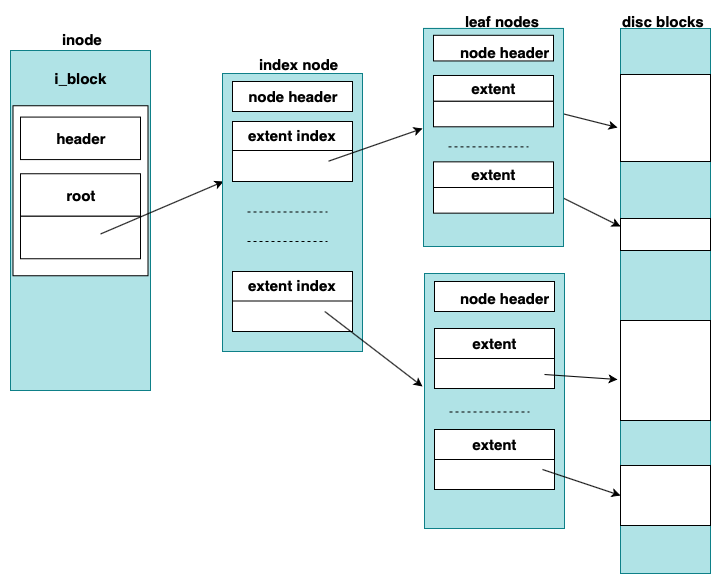
\includegraphics[width=.40\textwidth]{images/extent_tree-2.png}
\caption{Extent Tree}
\label{fig:extenttree}
\end{figure}

%Due to the block-oriented nature of most storage devices, conventional file systems have been designed with block-oriented indexing structures, such as extent tree in Linux Ext4 file system. Extent tree is suitable data structure to map the sequentially allocated blocks, so called as Extent, and to optimize the asymmetric sequential and random access latency of block-based storage devices. However, with the arrival of emerging NVM technology, it paves way for managing storage area with fine-grained granularity and making use of memory-oriented indexing structures in designing file systems.

In this project, we replace extent trees in Strata with two different hashing schemes described in sections \ref{Background}, namely Bucketized Cuckoo Hashing (BCH) and Level Hashing.

Strata makes use of extent trees to index blocks for each inode, which are digested from LibFS's private NVM log area to KernelFS's shared NVM space. As shown in Figure~\ref{fig:extenttree}, the existing allocator for the shared NVM space of KernelFS keeps a free list of 4KB block units and allocates contiguous blocks for digestion. Extent trees index these contiguously allocated blocks by using extents which store the starting physical address of the block and its size.

For the hash table implementation, we statically allocate blocks with 4KB granularity instead of assigning contiguous blocks, as shown in Figure~\ref{fig:hashtable}. The intuition behind this idea is that static allocation will reduce the overhead caused by merging and splitting fragmented blocks. In order to allocate blocks statically (with 4KB size), we divide the file size into 4KB chunks, and allocate NVM area separately for each.
%divide the digested file length by shifting its length with global block size implemented with \textit{length $>>$ g\_block\_size\_shift} in code lines and then those individual blocks are requested to be allocated in NVM shared area.

The root of the hash table is stored in each on-disk inode and is initialized when digesting the inode. The hash table stores the logical block number as the key and the physical block number are as its value. When digesting data blocks of a file, logical block numbers of a file inode are inserted into hash table with the corresponding physical block number given by the shared NVM allocator.

\begin{figure}[t]
\centering
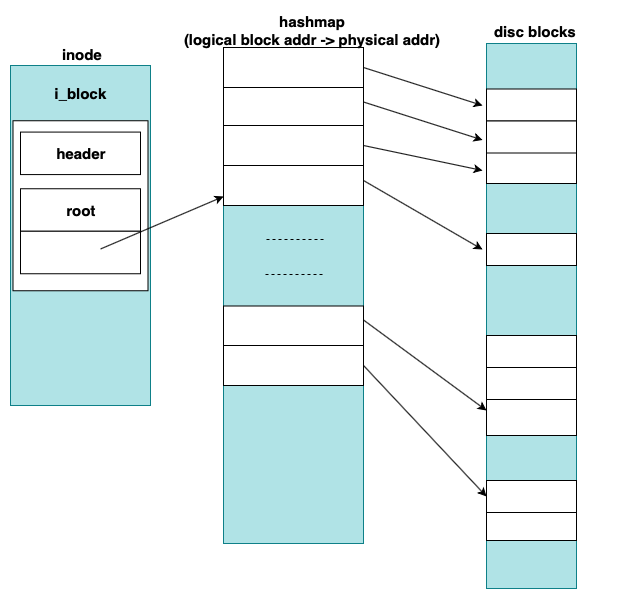
\includegraphics[width=.33\textwidth]{images/hash_table-2.png}
\caption{Hash Table}
\label{fig:hashtable}
\end{figure}

The hash table for each file is initialized to level size 4 which means, it will store $2^4$ top-level buckets and $2^3$ bottom-level buckets in the case of level hashing, and $2^4$ slots for BCH. This is a reasonable trade off as we are not wasting much space for small size files while also ensuring that the number of collisions is reduced. When the table is filled and new value is unable to be inserted into it, the hash table is resized, and the pointer to the new location is updated in the inode. The inode is subsequently marked dirty and hence the changes are persisted onto the disk. LibFS will modify its in-memory inode by reading this up-to-date on-disk inode, when it accesses the shared NVM area for traversing the hash table.

The original implementation of both BCH and level hashing allocates memory using heap memory allocators such as \textit{malloc}. However, this does not work in KernelFS when the data has to be stored in the NVM's shared area. Hence, we use the API provided by Strata to get free blocks in NVM's shared area for storing the hash table. In contrast to the individual file block allocation discussed above, the hash table blocks are contiguously allocated. It makes hash table cache-friendly and reduces the bookkeeping required to handle the blocks.
%The existing implementation of BCH and level hashing used a string based hash function to store integer-based block numbers, which resulted in high overhead during integer-to-string and string-to-integer conversions. Converting the hash table to directly take in integers, resulted in removing the overhead of string-copy and string-compare operations, leading to better performance.
% The existing implementation of BCH and level hashing is based on string 16-byte key and 15-byte value pairs~\cite{git_levelhashing}. However, it can cause high conversion overhead of string-to-integer and integer-to-string if we apply it as-is to index the logical block number and physical block number whose types are integers. Therefore, we change the string-based original implementation to support integer type key-value pairs. Although it is minor implementation issue, we can achieve the performance improvement by removing the overheads caused by the string copy operations and the string comparison operations as well as the key conversion overhead.
\begin{figure}[t]
\centering
\includegraphics[width=.35\textwidth]{images/micro_1MB.pdf}
\caption{Microbenchmarks with 1MB I/O}
\label{fig:micro_1mb}
\end{figure}

To guarantee data consistency of updating extent tree stored in the shared NVM area, the original implementation of Strata tracks the structural updates of extent tree by using buffer heads that are in-memory and then synchronize its updates by replaying the update information listed in buffer heads. It is the general way to load data stored in slow block-oriented storage into memory and then synchronize the updates made in the memory into persistent storage. It is necessary for slow block storage units, as the updates are time consuming and batching helps in reducing the latency~\cite{tweedie1998journaling,axboe2004linux}. However, it is unnecessary for NVM-based systems as NVM has low access latency, similar to DRAM, and can be accessed with byte granularity. Therefore, instead of using buffer heads, we directly synchronize the updates of hash tables into the shared NVM area by persisting the changes to ensure consistency. 
\vspace{-0.3cm}
\section{Evaluation} \label{evaluation}
\vspace{-0.2cm}
In this section, we evaluate our Level-hashing based Strata and Cuckoo hash based implementation\footnote{\url{https://github.com/SeKwonLee/strata}}. To test the effectiveness of our modifications, we compare their performance with the original Strata based on Extent tree. The experiments are run on a workstation with Intel(R) Xeon(R) CPU E3-1225 v5 3.30GHz and 32GB DRAM running the Linux kernel version 4.8.12. We compile all implementations using GCC-5.5.0. We reserve 16GB of DRAM to emulate NVM. Among this reserved DRAM, Strata allocates 256 MB for the private NVM log area of LibFS and 10 GB for the shared NVM area of KernelFS. We intentionally assigns the size of the private NVM log area to be small in order to generate frequent digestions. All experimental results are the average throughput of three repeated runs.

\subsection{Microbenchmark}
To compare the performance of each file system operations, we measure the performance of Sequential Write (SW), Sequential Read (SR), Random Write (RW), and Random Read (RR) on a 1GB file while changing I/O granularity. Figure~\ref{fig:micro_1mb} and Figure~\ref{fig:micro_1kb} shows the performance of each file system operations when using 1MB and 1KB I/O size respectively.

\begin{figure}[t]
\centering
\includegraphics[width=.35\textwidth]{images/micro_1KB.pdf}
\caption{Microbenchmarks with 1KB I/O}
\label{fig:micro_1kb}
\end{figure}

The first thing we notice is that 1MB I/O gives better performance as compared to 1KB for all designs. This is due to the fact that every time a block is needed to be accessed, LibFS has to go through KernelFS to get the physical block location from hash table/extent tree. Even in the original implementation of Strata where the extent cache is present, only the path is stored in it, and the actual data still have to be retrieved from the extent tree. This kernel access bogs down the performance for the 1KB I/O case.

We can see that the extent tree implementation performs relatively better as compared to the hash table for sequential write. This is to be expected as sequential writes for extent trees will need only contiguous memory to be allocated and the extents to be formed. The overhead of having to allocate each block of memory independently is reducing the performance of the hash table implementation.

Sequential read performs better with extent tree for 1MB I/O and with hash table for 1KB I/O. This is a good example to look at, to understand the tradeoff between extent tree and hash maps. Since the number of read calls are lesser for 1MB I/O, the number of extent tree searches are small and hence the access is quick enough to outperform hash tables. But once we move into higher number of queries to the extent tree, the higher search time in extent tree compounds as compared to hash map.

The performance of both schemes in the case of random read can be explained similarly as above. We can notice that hash tables gives almost par performance even for 1MB I/O case here. This follows from the fact that random reads might need more than one extent to be accessed, leading to increased search time, while hash tables don't have any impact in its retrieval performance.

Hash tables perform better for random writes for 1MB I/O case as well. This is to be expected given that the extents mapping to the memory chunk being overwritten might be from two different extents as before. This will result in more time traversing the extent tree. Hash table on the other hand will give the relevant addresses in constant time, and since there is no overhead of the memory having to be allocated for each block (as with sequential write where the file is being created from scratch, instead of data just being overwritten like here), it outperforms extent tree design. We were unable to run evaluation for random write for 1KB I/O case, as the original Strata implementation was failing for the same.

\begin{figure}[t]
\centering
\includegraphics[width=.35\textwidth]{images/fileserver.pdf}
\caption{Fileserver}
\label{fig:fileserver}
\end{figure}
\vspace{-0.3cm}
\subsection{Macrobenchmark}
We performed experiments with filebench by using fileserver and webserver workloads. Fileserver is write-intensive (write:read=2:1) and webserver is read-intensive (write:read=1:10). Both workloads operate on a working set of 10,000 files. The average size of files is 128KB and 16KB for fileserver and webserver respectively, while files are appended via 16KB. We run each workload for two different I/O sizes of 1MB and 1KB.

As we can see in Figure~\ref{fig:fileserver}, hash tables give better performance for fileserver with 1MB I/O. The workload of fileserver includes file unlink operations in addition to write and read operations. In the extent tree based implementation, they cause NVM space to be fragmented as the freed data blocks can leave holes between contiguously allocated blocks. This results in additional overheads for fragmentation management such as finding sequential empty spaces and merging extents together. However, the hash table designs are not vulnerable to it as they manage NVM space with finer granularity by only using 4KB blocks. In case of the result with 1KB I/O, Extent tree shows comparable performance with hash tables. It is because the overhead of block rearrangement caused by fragmentation can be avoidable when the requested I/O size is lower than 4KB block.

\begin{figure}[t]
\centering
\includegraphics[width=.35\textwidth]{images/webserver.pdf}
\caption{Webserver}
\label{fig:webserver}
\end{figure}

Figure~\ref{fig:webserver} shows the performance of webserver workload. Extent tree achieves significant improvement compared to the hash table in 1MB I/O. This is due to the difference in the number of index searches required to obtain the requested block. Extent tree requires only one traversing to get 1MB large block while multiple accesses are inevitable for the hash tables indexing the individual 4KB blocks. For small size I/O, both extent tree and hash table are required the equal number of searches. Therefore, hash tables that have the constant search time show better performance than extent tree.


% \section{Related Work}
% \subsection{Tree-based structures for NVM}
% Most of the work in this area focuses on B-trees \cite{bplustree}. Chen et al. \cite{PCM} proposed a B+ tree indexing structure for Phase Change Memory (PCM) that
% reduces PCM writes without considering the data consistency of
% B+ tree in PCM. Venkataraman et al. \cite{CDDS} proposed the
% CDDS B-tree that leverages versioning, \textit{CLFLUSH} and
% \textit{MFENCE} instructions to achieve data consistency in Btree.
% Yang et al. \cite{NV-Tree} proposed the use of NV-Tree to guarantee
% the consistency of only leaf nodes in B+-tree while
% relaxing that of internal nodes. The internal nodes can
% be reconstructed based on leaf nodes in case of system failures.
% NV-Tree reduces the number of cache line flushes since it
% only persists the leaf nodes. Apart from B-tree indexing structures, Lee et al. \cite{WORT} focuses on using radix tree in persistent memory and proposes Write Optimal Radix Trees (\textit{WORT}) that achieve data consistency via 8-byte atomic writes.

% \subsection{Hashing based structures for NVM}
% PFHT \cite{PFHT} and path hashing \cite{pathhashing}, mainly focus
% on reducing NVM writes without considering the consistency issue in NVM. Level Hashing \cite{levelhashing} guarantees the consistency of hash table
% through log-free schemes, while giving high performance and rarely incurring extra NVM writes. The resizing operation in hash
% tables is expensive for the tolerance and performance of
% NVM systems, which only Level Hashing considers.

\section{Conclusion} \label{conclusion}
\vspace{-0.2cm}
We have found out that the hash tables give better performance for finer granularity I/O operations, due to faster search times. They are also more efficient in write and delete intensive workloads due to their fragmentation immunity. The modified model performs $4.8\%$ better in filebench fileserver benchmark and outshines the original implementation in random read and write microbenchmarks.

\bibliography{citations}
\bibliographystyle{ieeetr}

\end{document}
